\section{Background and Related Work}
\subsection{\acf{RE} of Autonomous Systems}
While static verification, such as timing verification, has its place, more dynamic approaches to verification and safety can be used to catch anything that the static verification may have missed.
Take a standard image classification \ac{CNN} for example.
The \ac{CNN} can be trained to 99.9\% accuracy according to the test cases used to train it.
However, this means that the \ac{CNN} fails 0.1\% of the time, and that is only on the tested population, not even taking the entire population into consideration.
Having a method to verify this \ac{CNN} while it is running and pick up any inevitable failures would allow for this \ac{CNN} to be used in systems where safety is critical.

\subsubsection{\acf{RV}}
\begin{figure}[h]
	\centering
	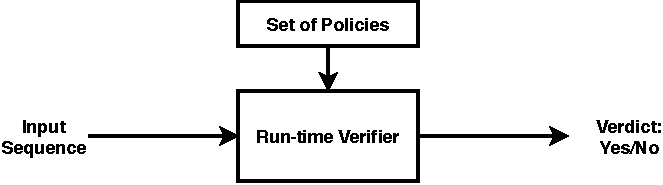
\includegraphics[width=0.6\linewidth]{Content/fig/RV-basic.pdf}
	\caption{Basic view of a run-time verifier. \label{fig:rvbasic}}
\end{figure}

Run-time verification is an extension of run-time monitoring~\cite{runtime-verify}.
A run-time verifier monitors the I/O events of a system using a specified safety policy.
The verifier provides positive or negative feedback depending on the I/O of the system, providing a verdict for the current state of the automaton.
The run-time verifier has no knowledge of the inner workings of the system, regarding it as a black box.
This makes it ideal for autonomous systems, where the inner workings are often too complex to be verified.
Figure~\ref{fig:rvbasic} shows the basic structure of a run-time verifier.

\subsubsection{\acf{RE}}
\begin{figure}[h]
	\centering
	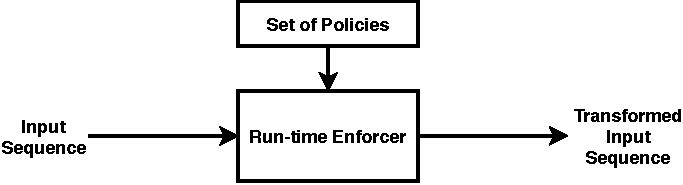
\includegraphics[width=0.6\linewidth]{Content/fig/RE-basic.pdf}
	\caption{Basic view of a run-time enforcer. \label{fig:rebasic}}
\end{figure}

\acf{RE} is a subset of \ac{RA} that focuses on formal semantics and blocking, delaying, modifying and/or re-ordering of events in a system. 
\ac{RE} can be transformation or reactive.
Transformational \ac{RE} uses the delaying, buffering and reordering of event to enforce a safety policy, while reactive \ac{RE} uses edit functions to edit events and can be bi-directional.
This paper focuses on reactive \ac{RE}, since \acp{ANN} are reactive in nature.
Processes that are deemed unsafe can be monitored by an enforcer at runtime to ensure that they obey desired policies and remain in a safe state at all times~\cite{theoryRE}. 
Formal runtime verification methodologies mathematically guarantee the detection of improper system behaviour \cite{RuntimeAssuranceForComplexCPS}.
For example, \ac{SA} have been proposed, which formally monitor uni-directional run-time properties only (e.g. outputs only)~\cite{enfsafepol}.
Edit automata are a type of \ac{SA} that can edit, suppress or insert events~\cite{editautomata}. 
\ac{DTA} have been proposed that can edit \textit{bi-directional} events at runtime~\cite{recps}. 
They were designed for reactive \ac{CPS} demonstrated in a pacemaker environment~\cite{recps}. 
Figure~\ref{fig:rebasic} shows the structure of a run-time enforcer.

\subsubsection{\acf{DTA} for \acf{RE}}
In order to specify the safety policies to be enforced by the run-time enforcer Pinisetty et al define \acf{DTA}~\cite{recps}.
These \ac{DTA} can be used to represent safety policies $\varphi$ which can be enforced at run-time using \textit{edit functions}~\cite{recps}.

Run-time enforcers are able to enforce binary I/O events at run-time.
I.e. the enforcers can enforce the absence or presence of an input or output signal at run-time.
A unique property of \ac{DTA} is their ability to express timed properties which can be enforced by a run-time enforcer.
A \ac{DTA} can have one or more timers, which increment at each discrete time instance.
Guards and transitions can be enforced that check the timer.
An example \ac{DTA} is given in Example~\ref{ex:dta} to introduce the syntax used in the \acp{DTA}.

\begin{figure}[h]
	\centering
	\includegraphics[width=\linewidth]{avdta.tikz}
	\caption{\ac{DTA} example showing the syntax used to describe \acp{DTA} in this paper\label{fig:avdta}}
\end{figure}

\begin{example}[Syntax of a \ac{DTA}]\label{ex:dta}
	The \ac{DTA} shown in Figure~\ref{fig:avdta} represents a basic safety policy.
	The policy as inputs A, B and C and output O and starts in the safe state $l_{safe}$.
	The policy's safe state transitions are described in layman's terms below: \\
	While A and B, denoted as $A~\&~B$ and not to be confused with A OR B ($A~|~B$), are present simultaneously, transition back to the safe state.\\
	However, if A and B are not detected simultaneously, transition to the unsafe state $l_{unsafe}$, suppress the output signal O ($O~:=~0$) and set the timer to 0 ($t~:=~0$).\\
	The statement ``$\sum\textbackslash~Z$'' reads as ``anything except Z''.
	The enforcer actions are indicated by statements using the syntax ``$X~:=~Y$'', which reads ``set X to Y''.\\
	\\
	The unsafe state has the following transitions:\\
	If the timer is less than 3 and C is not been present, transition back here while suppressing output 0.\\
	If the timer is greater than, or equal to, 3 and C is not been present, transition to the safe state.\\
	If C is detected, transition to the violation state.\\
	The absence of a signal is detected using the \textbf{overline}, e.g. ``not X'' would be $\overline{X}$.\\
	\\
	The violation state has only a single transition that returns to the violation state on anything.\\
	\\
	A brief description to the \ac{DTA} would be to say the A and B must be present together. 
	If they are not, the system is unsafe for 3 ticks, within which if C is present a violation occurs.
	After 3 ticks, the system returns to a safe state.
	While the system is in the unsafe state, the output O is suppressed by the enforcer.
\end{example}

\subsection{\acfp{ANN} for \acf{CPS}}
In order for an \ac{ANN} to be used in any capacity within a system where safety is critical, it should undergo rigorous and thorough validation, verification, and testing procedures to ensure that they it is sufficiently safe for its target system~\cite{scann, ANNSafetyLifecycle2003}. 

While considerable research effort is starting in the direction of formal verification of \ac{AI}-based \ac{CPS}~\cite{seshia2016towards, russell2015}, the issue of timing verification has received scant attention. 
Like the challenges involving functional verification, timing verification of AI-based  \ac{CPS} poses considerable challenges due to the fact that: (1) real-time \ac{AI} systems could involve many concurrent and interacting \ac{AI} modules, which need deterministic composition for safety; (2) \ac{AI} modules are usually developed as untimed systems and the reactive nature of AI algorithms used in CPS are not carefully studied; and (3) \acf{WCET} analysis~\cite{wilhelm2008worst} of \ac{AI}-based \ac{CPS} has received scant attention.

Definitions for this safety vary, but Kurd et. al.~\cite{EstSafeCriteria2003} provide a generalisation: safe \acp{ANN} can be defined as those that:
\begin{itemize}
	\item tolerate faults and inconsistencies in their inputs,
	\item do not create hazardous outputs,
	\item behave in a predictable and repeatable manner,
	\item and are trained on clean, reliable data. 
\end{itemize}

To achieve these properties, there exist safety measures such as risk management systems that span the entire development process of the \ac{ANN}~\cite{ANNDevModel1999} and standards with which \acp{ANN} can be certified before they are used in systems where safety is critical~\cite{SCANNStandard}. 
These techniques are primarily \textit{proactive} in nature, producing \acp{ANN} that are classified as \textit{safe enough} for their role. 

However, as \acp{ANN} become larger and more full-featured, they  become harder to statically analyse.
Problematic situations can arise when an \ac{ANN} exhibits unexpected behaviour that the system is unable to safely respond to, and in \ac{CPS} these situations can be life threatening.

\subsection{Functional Verification of \acfp{ANN}}
Typical approaches for ensuring that \acp{CPS} are safe involve processes to demonstrate that an acceptable level of risk has been achieved~\cite{scann}. 
Designers of \ac{AI} software rely on several validation and verification technique, including, but not limited to, conventional testing, run-time monitoring, static analysis, model checking and theorem proving~\cite{menzies2005verification}.
Unfortunately, due to the complexity of \acfp{ANN}, techniques such as static analysis, model checking and theorem proving are less valuable in \ac{ANN} environments. 
Conventional testing is a common method to test the accuracy of \acp{ANN}, but this method is not fool-proof and its efficacy relies heavily on the creator of the test cases.
Run-time monitoring is a technique that could greatly benefit the safety of running \acp{ANN}, but there has been minimal research done in this field.

There are a variety of pre-existing methods for statically checking the correctness of autonomous (i.e. artificially intelligent) systems.
For instance, model checking on systems that use timed automata~\cite{timed-enf-autonomous}.
Okano et. al. explore the concept of model checking of autonomous systems that use timed automata~\cite{timed-enf-autonomous}.
Conventional model checking done on this automaton allowed the safety and robustness of the system to be demonstrated.
While techniques such as model checking work very well on non-\ac{ANN} \ac{AI}, \acp{ANN} are not usually able to be simplified to simple automata. 
This technique is a static technique and cannot be applied to autonomous \ac{ANN} systems, where the behaviour of the \ac{ANN} controller cannot be defined by an automaton.
For an autonomous system that includes at least one \ac{ANN} in its controller, novel techniques are required to guarantee the safety properties of the \acp{ANN}.
However, \acp{ANN} are not usually able to be simplified to simple automata.

Deep learning is a widely and extensively researched field with regards to modern machine learning that refers to the learning of data representations, rather than learning task specific algorithms~\cite{schmidhuber2015deep}.
Deep learning has applicability in a lot of current \ac{ANN} implementations, such as the autonomous vehicles used by Tesla and Uber.
Verification of \ac{ANN}, specifically, Deep Neural Networks, can be performed for certain properties (such as robustness) using \ac{SMT}~\cite{Gehr2018AI2SA,DeepANNverify,reluplex}.
This is useful, because the robustness of a deep \ac{ANN} is a critical property of its safety.
A robust \ac{ANN} is one that will provide consistently accurate outputs even when the input to the \ac{ANN} is noisy, incorrectly coloured or otherwise distorted. 
However, this approach is not flawless. 
\ac{SMT} has issues with scale: as the \acp{ANN} to analyse become larger, analysis time grows exponentially~\cite{Gehr2018AI2SA}.
Ergo, they are less efficient on larger, more complex \acp{ANN}.
In addition, they require the \acp{ANN} to fulfil some specific properties, such as specific activation functions and specific \ac{ANN} variants, i.e. \cite{Gehr2018AI2SA} only allows \acp{CNN} and \acp{MLP} with \ac{ReLU} activation functions.
This limits flexibility, as each \ac{ANN} must be designed around these restrictions, thus limiting properties of the \ac{ANN}, such as its activation function and size, could result in an \ac{ANN} that is inefficient, not robust, slow, etc.

Due to these difficulties, it can be tempting for designers to simply rely on manual testing to check for the correctness of \ac{ANN}-based systems. 
However, this is a time-consuming and error-prone process which cannot provide good guarantees, as it is very difficult to ensure that tests have acceptable coverage of all possible situations~\cite{ANN-test}.
Furthermore, as with the static analysis approaches, as the \acp{ANN} increase in size and complexity, verification and validation of these networks becomes increasingly more difficult to achieve~\cite{Gehr2018AI2SA}; test data is not unlimited, time is a resource and verification is not 100\% accurate.

Finally, no matter the chosen methodology, as \acp{ANN} increase in size and complexity, verification and validation of these networks becomes increasingly more difficult and resource intensive to achieve~\cite{Gehr2018AI2SA}.

\subsubsection{\acf{RE} of \acfp{ANN}}
% Write about exisiting autonomous RE
The idea of \ac{RE} of autonomous systems has received some research attention. 
De Niz et. al. propose a type of \ac{RE} they term temporal enforcement, which ensures that the system controller meets timing deadlines where outputs are concerned~\cite{safe-enforce-auto}. 
While this shares similarities with the work in this paper, their work does not expand to cover \acp{ANN}, and does not propose the use of \ac{RE} for anything other than meeting timing deadlines.
Aniculaesei et. al. propose static formal verification and runtime monitoring of autonomous, robotic systems to prevent physical collisions during system execution~\cite{runtime-monitor}.
While this looks at the enforcement of system outputs, the inputs are not monitored and the timing deadlines of the system are not investigated. 
Additionally, the case study involves a robot controlled by an automaton, not a highly complex \ac{AI} such as an \ac{ANN}.
